%!TEX root = ../dissertation.tex
\chapter{Autodiagnostica di anomalie}
\label{AutodiagnosticaDiAnomalie}

Questo capitolo tratta l'addestramento di vari algoritmi di machine learning e la valutazione di essi, tratta inoltre il processo di feature extraction applicato ai dati prima di essere utilizzati.

\section{Feature extraction}
Nell'ambito del machine learning con feature extraction si intende l'estrazione di caratteristiche dai dati di ingresso per semplificare in seguito l'apprendimento.
L'estrazione di feature è particolarmente utile quando il numero di dati in ingresso all'algoritmo di machine learning è molto alto, e renderebbe l'apprendimento troppo lungo e complesso \cite{FeatureExtraction}.

A seconda dei dati e il loro contesto ci sono molti metodi di estrazione di feature. Per le immagini si usano algoritmi che cercano e riconoscono caratteristiche come linee, angoli e contorni all'interno della figura e queste caratteristiche vengono usate per il machine learning invece dell'immagine completa che spesso contiene molte informazioni ridondanti o poco utili, che rallenterebbero o renderebbero impossibile l'apprendimento.

I dati letti dai sensori del MPFM sono invece una serie temporale, ovvero una serie dove i dati sono legati all'istante di tempo in qui sono stati osservati, in questo caso alcune delle feature che si possono estrarre sono minimo e massimo globale, numero di "picchi" ovvero minimi e massimi locali, media, mediana, varianza, deviazione standard. In questo modo si riduce il numero di dati da centinaia di migliaia di punti a un decina di caratteristiche fondamentali che riassumono adeguatamente cosa è accaduto in quella particolare porzione di tempo.  

Nel caso del Multiphase Flow Meter alcuni dei sensori effettuano fino a 2500 letture al secondo, e in un solo minuto di registrazione si ottengono già 150000 valori per uno solo delle 20 o 30 variabili lette dai sensori presenti nel MPFM. Per questo motivo prima di allenare un algoritmo di machine learning bisogna estrarre alcune delle feature più rilevanti da questi dati. 

\subsection{tsfresh} \label{tsfresh}
tsfresh è la libreria utilizzata per l'estrazione di feature in quanto specifica per le serie temporali, come per le letture dei sensori del MPFM \cite{tsfresh}.

tsfresh permette quindi di calcolare automaticamente un certo numero di feature su una serie temporale qualsiasi. Sono presenti più di 100 feature estraibili con tsfresh ma estrarle tutte richiederebbe troppo tempo e spesso risultano ridondanti in questo contesto.

\begin{figure}
	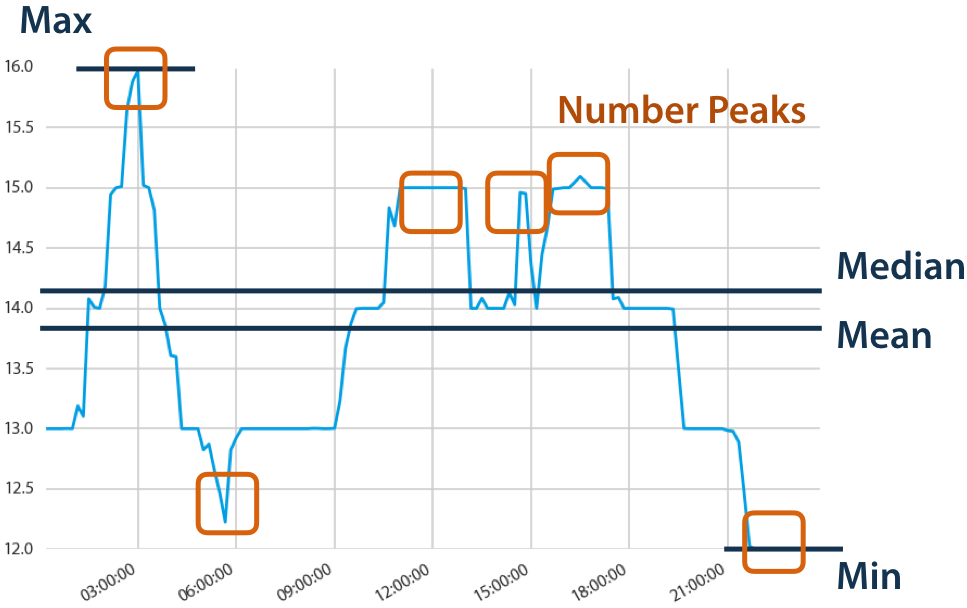
\includegraphics[width=\textwidth]{figures/tsfresh_features}
	\caption[Esempio di feature estratte dalla libreria tsfresh]{ Esempio di alcune feature estraibili da una serie temporale attraverso la libreria tsfresh
		
		\label{fig:tsfresh_features}}
\end{figure}

Si è scelto quindi un set ridotto di feature che comprende solamente le seguenti caratteristiche per ogni minuto di letture di dati:

\begin{itemize}
	\item Minimo
	\item Massimo
	\item Media
	\item Mediana
	\item Deviazione standard
	\item Varianza
\end{itemize}

Minimi e massimi permettono di riconoscere valori troppo alti o bassi per essere letture reali sullo stato del flusso, ad esempio letture di pressione e temperature che risultano fisicamente impossibili e possono essere quindi categorizzate come anomalie nel funzionamento dello strumento. Media e mediana forniscono un punto di riferimento sui valori normali per quel minuto di lettura. Deviazione standard e varianza possono dare informazioni sul regime del flusso, varianza molto alta potrebbe essere causata da un flusso turbolento dove i valori letti cambiano notevolmente da secondo a secondo, allo stesso modo bassa varianza può indicare un flusso più costante.

Inoltre selezionando solo 6 feature il tempo di estrazione si riduce drasticamente, ma rimane comunque notevole quando lo si deve applicare per ogni minuto di lettura in migliaia di file raw.
Per non ripetere l'estrazione di feature ogni volta che si vuole applicare un algoritmo di machine learning, è stata effettuata l'estrazione delle feature di tutte le variabili di tutti i file raw una volta sola e il risultato è stato salvato in una tabella apposita nel database. Questo processo ha richiesto circa 8 ore per il completamento, ma una volta presenti nel database le feature si possono ottenere istantaneamente.

\section{Anomaly detection}

L'anomaly detection consiste nella identificazione di osservazioni o eventi che differiscono sostanzialmente dalla maggior parte degli altri dati. Nel contesto del Multiphase Flow meter queste anomalie nei dati possono corrispondere a dei problemi o difetti nello strumento o nei sensori stessi. Per questo motivo individuare le anomalie attraverso algoritmi di machine learning può essere utile per diagnosticare lo stato dello strumento, e in alcuni casi prevedere quando si sta per rompere prima che accada.

Esistono due tecniche principali di anomaly detection. L'anomaly detection supervisionato richiede che i dati siano classificati come "normali" oppure "anormali" e sfrutta questa proprietà per classificare i nuovi dati dopo l'apprendimento. L'anomaly detection non supervisionato non richiede nessuna classificazione dei dati e assume che la maggior parte dei dati siano normali e cerca i punti  meno simili agli altri \cite{AnomalyDetection}.

Le letture effettuate dei sensori durante i test non sono classificate quindi è necessario usare un approccio non supervisionato. 

\subsection{scikit-learn e PyOD}
scikit-learn\cite{scikit-learn} è una libreria che offre una vasta quantità di strumenti e funzioni per machine learning in Python, tra i quali implementazioni degli algoritmi più comuni, metodi per estrarre feature e normalizzare i dati e molto altro.
PyOD\cite{zhao2019pyod} invece è una libreria più semplice, specifica per lavorare nel campo dell'anomaly detection e spesso sfrutta alcune delle funzionalità offerte da scikit-learn.

Da queste librerie sono stati scelti 5 degli algoritmi più utilizzati per l'anomaly detection e sono stati valutati e confrontati tra loro.

\subsection{Histogram-Based Outlier Detection (HBOS)}
In questo algoritmo viene costruito un istogramma per ogni variabile e la combinazione di tutti gli istogrammi viene utilizzata per determinare quali punti sono "outlier" ovvero anomalie. Questo algoritmo assume che i data normali siano concentrati in una particolare zona e non performa altrettanto bene se i dati sono divisi in diversi cluster. In compenso è uno degli algoritmi più efficienti e classifica i dati in tempo lineare O(n) oppure O(n*log(n)) a seconda se il "bin size" è statico o dinamico \cite{HBOS}.

\subsection{Isolation Forest}
Isolation Forest è un algoritmo che si concentra su isolare le anomalie che sono definite come i punti più rari e isolati. In breve una foresta di alberi binari di ricerca è costruita seguendo un approccio che divide casualmente in due lo spazio dei punti. Ad ogni iterazione ogni parte è divisa a sua volta in due fino a quando contiene un solo punto. I punti più isolati saranno separati dagli altri in un minor numero di tagli e saranno quindi più vicini alla radice dell'albero binario. A tutti i punti viene quindi assegnato un punteggio in base alla loro altezza nell'albero, dove le anomalie avranno punteggio più alto in quanto sono più vicine alla radice e i punti normali un punteggio più basso in quanto più distanti dalla radice \cite{IF}.


\subsection{K-Nearest Neighbors (KNN)}
Questo algoritmo si basa sulla distanza di ogni punto dai suoi k punti più vicini per determinare gli "inlier" e gli "outlier" ovvero i punti normali e le anomalie\cite{KNN}. Il punteggio di anomalia può essere calcolato attraverso tre metodi differenti: 	
\begin{itemize}
	\item "largest": usa la distanza maggiore tra tutti i k vicini come punteggio di anomalia
	\item "mean": usa la media delle distanze dai k vicini come punteggio di anomalia
	\item "median" usa la mediana delle distanze dai k vicini come punteggio di anomalia
\end{itemize}
Sono state effettuate più prove con configurazioni diverse di questo algoritmo, la più efficace per riconoscere le anomalie nei dati dei sensori e quella che è stata utilizzata nei confronti tra gli algoritmi è stata utilizzare 5 vicini e calcolare il punteggio attraverso il metodo "largest".

\subsection{Local Outlier Factor (LOF)}
Local Outlier Factor è un algoritmo basato sul confronto tra la densità di un punto e la densità dei suoi punti più vicini. Considera quindi come outlier i punti che hanno minor densità rispetto ai loro punti più vicini. Similarmente a KNN la densità è calcolata in base alla distanza di un punto ai suoi vicini, solo che il punteggio di anomalia non viene ricavato dalla distanza stessa, ma da quanto diversa è la densità del punto rispetto alle densità dei suoi k vicini.
La località dell'algoritmo permette di riconoscere anomalie che non sarebbero considerate da altri algoritmi, ma questo approccio spesso è applicabile solo a spazi di dati con poche dimensioni \cite{LOF}.
Il valore di k scelto per questo algoritmo è 20, in base a più prove con valori più o meno alti che hanno ottenuto risultati simili o peggiori.

\subsection{Principal Component Analysis (PCA)}
A differenza dell'Isolation Forest questo metodo cerca di classificare gli "inlier" e considera i punti rimanenti come anomalie. Spesso è utilizzato quando si lavora con spazi di dati a molte dimensioni, oppure quando il numero di anomalie è basso e classificarle risulta più difficile di classificare i punti normali. PCA determina quale caratterista ha il maggior impatto sulla varianza dei dati, ovvero determina le componenti principali \cite{PCA}.

\subsection{Addestramento e confronto} \label{AddestramentoEConfronto}

Per l'addestramento degli algoritmi sono state utilizzate le feature estratte in precedenza e caricate nel database. Si ricorda che le feature scelte in sezione \ref{tsfresh} sono: massimo, minimo, media, mediana, varianza, deviazione standard di un minuto di dati. Ogni confronto è stato ripetuto per 3 variabili differenti, in particolare sono state utilizzate C1\_V71\_0 che misura la capacità del fluido, C1\_V71\_1 che misura la resistenza del fluido, e NIR\_S1 che è uno dei sensori che misura il WLR.
Per la variabile C1\_V71\_0 sono stati utilizzati 5369 minuti di dati, questo numero corrisponde quindi al numero di sample usato nell'apprendimento. Per la variabile C1\_V71\_1 invece sono stati utilizzati 1122 sample, e infine per NIR\_S1 7267 sample.
La dimensione dei dati dipende dal numero di feature utilizzate, in questo caso è 6 per tutte e tre le variabili.

Non conoscendo quali dei punti sono veramente anomalie, o se i dati non contengono nessuna anomalia, si è deciso di aggiungere del rumore casuale entro il minimo e il massimo dei punti. I punti che formano il rumore possono essere quindi considerati come le anomalie da trovare. 

Di conseguenza ad ogni variabile è stato aggiunto un numero di punti casuale pari al 10\% del numero di sample iniziale. La valutazione di un algoritmo dipende dal numero di punti aggiunti casualmente classificati correttamente come outlier, e dal numero di punti originali classificati correttamente come inlier.

\begin{figure} [H]
	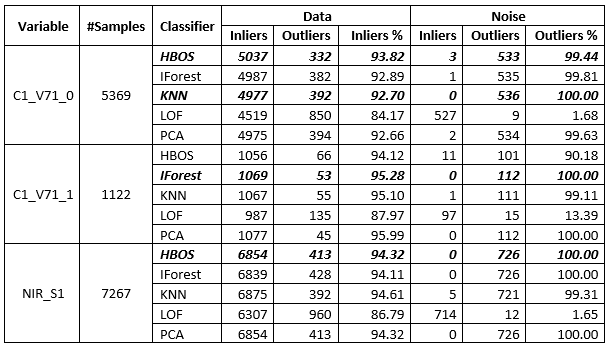
\includegraphics[width=\textwidth]{figures/homogeneous_noise}
	%\caption[Esempio di features estratte dalla libreria tsfresh]{
		
	%\label{fig:homogeneous_noise}}
\end{figure}

Dai risultati si può vedere come tutti gli algoritmi siano riusciti a classificare correttamente come outlier praticamente tutto il rumore, tranne per LOF che non ha riconosciuto il rumore come anomalia in nessuna delle tre variabili.

Infine l'addestramento è stato ripetuto con l'aggiunta di rumore non più omogeneamente, ma raggruppato in 5 cluster casuali.

\begin{figure} [H]
	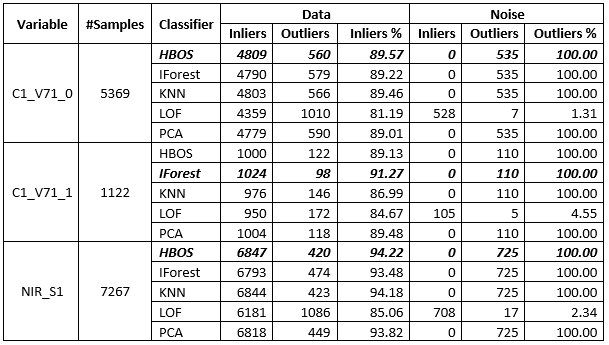
\includegraphics[width=\textwidth]{figures/cluster_noise}
	%\caption[Esempio di features estratte dalla libreria tsfresh]{
	
	%\label{fig:homogeneous_noise}}
\end{figure}

In questo caso tutti gli algoritmi hanno performato addirittura meglio, probabilmente perché il cluster erano troppo distanti dalla maggior parte dei dati e troppo poco densi per confondere gli algoritmi basati sulla densità. LOF non riesce ancora a distinguere correttamente il rumore, forse per una configurazione sbagliata nel momento dell'apprendimento.

\section{Visualizzazione delle anomalie}

Per verificare il funzionamento degli algoritmi, e avere un'idea sulla motivazione delle scelte effettuate dagli algoritmi nel momento della classificazione, sono stati creati dei grafici che mostrano i dati iniziali e la loro classificazione dopo l'addestramento.

Nei seguenti grafici è stato utilizzato l'algoritmo HBOS addestrato sulla variabile C1\_V71\_0. L'addestramento comprende tutte e 6 le feature utilizzate in precedenza, ma per poter creare un grafico in due dimensioni sono state utilizzate la deviazione standard nelle ascisse e la media nelle ordinate.

\subsection{Visualizzazione degli outlier}
Nel grafico in figura \ref{fig:vis1} i punti in rosso sono stati classificati come outlier, mentre quelli in verde come inlier. Anche se a prima vista il numero di outlier sembra molto maggiore degli inlier, dall'istogramma si può vedere che è esattamente il contrario. La maggior parte dei punti è altamente concentrata in una piccola zona, i punti lontani da questa concentrazione sono stati quindi classificati come anomalie.

\begin{figure} [H]
	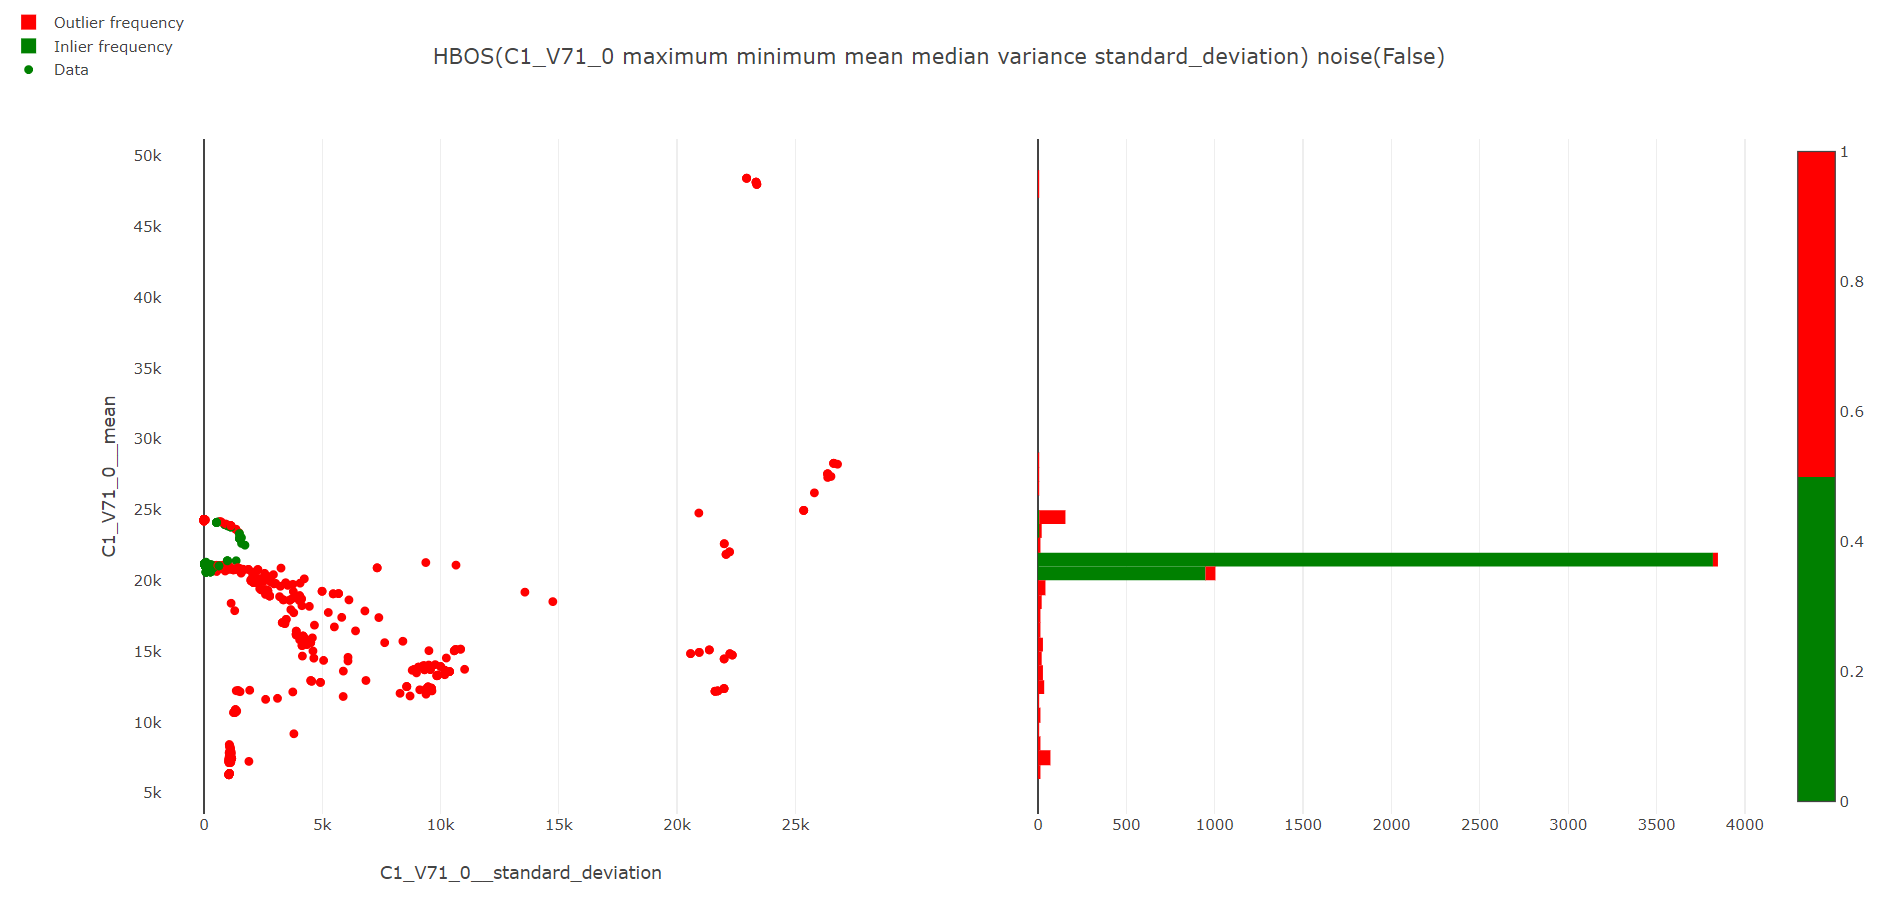
\includegraphics[width=\textwidth]{figures/vis1}
	\caption[Grafico dell'anomaly detection nella variabile C1\_V71\_0 con HBOS]{Grafico dell'anomaly detection nella variabile C1\_V71\_0 con HBOS. In rosso gli outlier, in verde gli inlier.
	
	\label{fig:vis1}}
\end{figure}

\subsection{Visualizzazione dello score dei punti}
A ogni punto viene assegnato uno punteggio o score in base dall'algoritmo utilizzato, questo punteggio è un valore da 0 a 1 che determina quanto sicuro è l'algoritmo nella classificazione del punto. In figura \ref{fig:vis2} si può vedere lo score di ogni punto in base al colore, i punti vicino al giallo sono più probabilmente outlier mentre i punti vicino al blu scuro sono più probabilmente inlier. In questo caso il colore dell'istogramma è irrilevante.

\begin{figure} [H]
	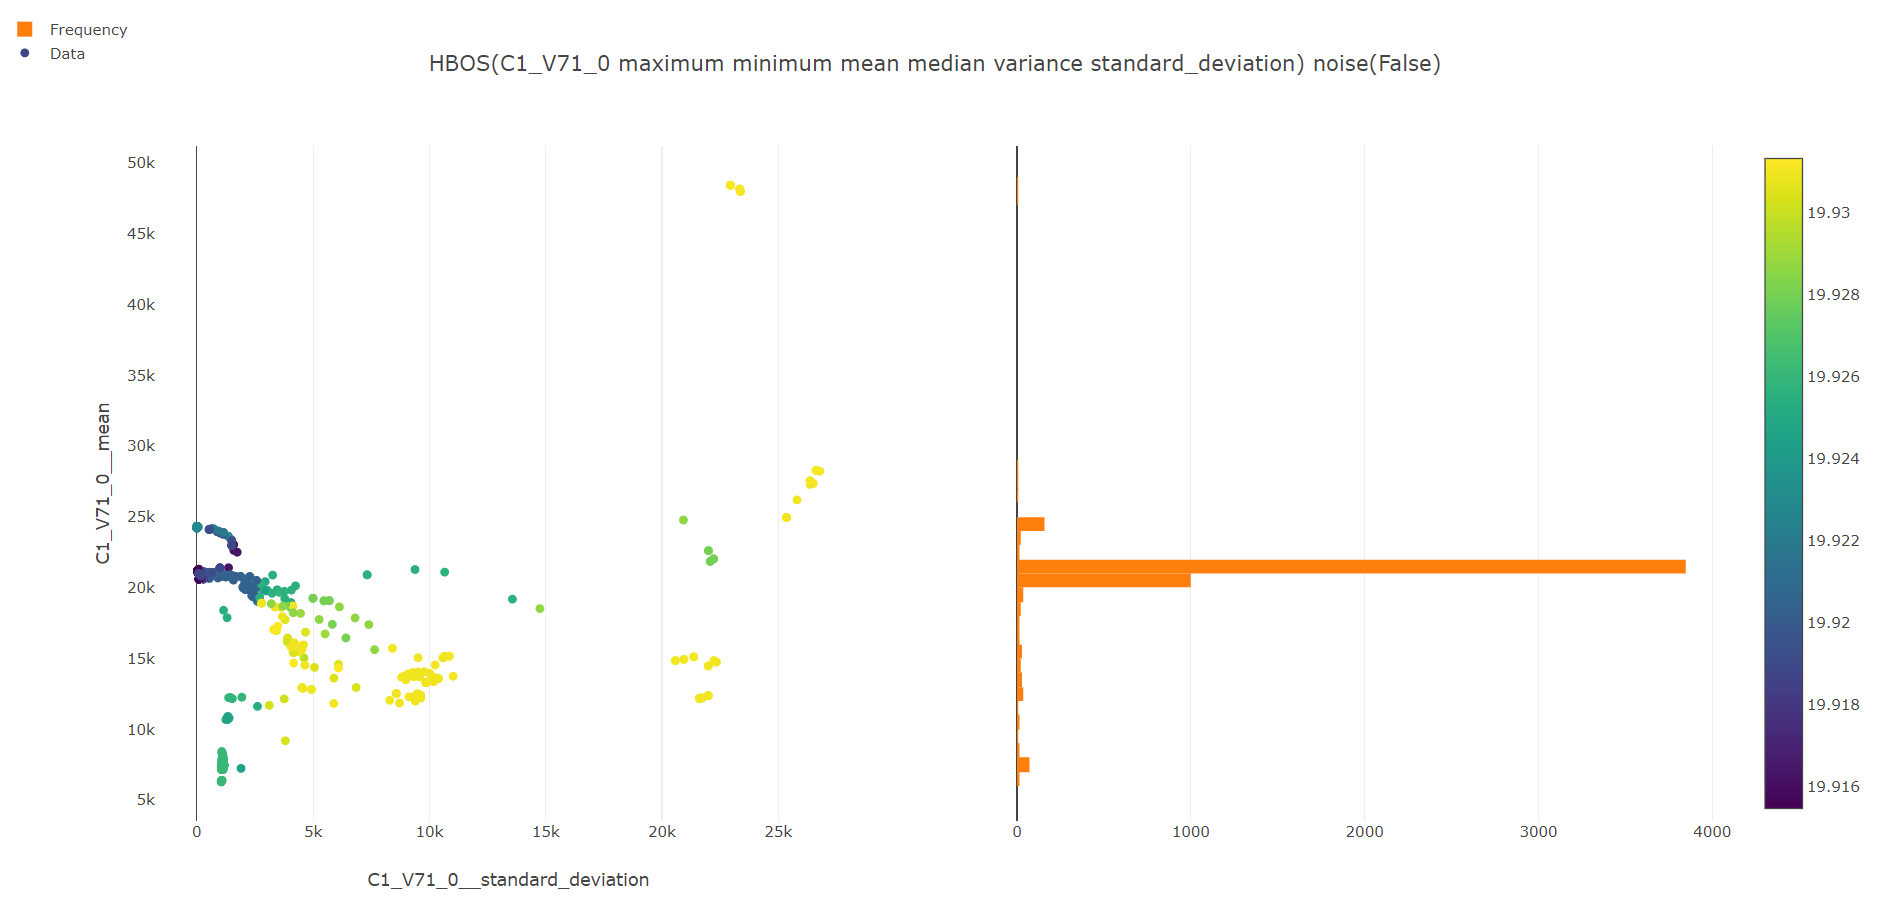
\includegraphics[width=\textwidth]{figures/vis2}
	\caption[Grafico dello score dei punti usando HBOS e la variabile C1\_V71\_0]{Grafico dello score dei punti usando HBOS e la variabile C1\_V71\_0. I punti verso il giallo sono più probabilmente outlier, mentre i punti verso il blu scuro sono più probabilmente inlier.
		
		\label{fig:vis2}}
\end{figure}

\subsection{Visualizzazione dello score con rumore omogeneo}
Nel grafico in figura \ref{fig:vis3} è stato aggiunto casualmente del rumore pari al 10\% dei punti iniziali. I dati iniziali sono rappresentati con dei pallini mentre il rumore con dei triangoli, tutti i punti sono colorati in base allo score assegnato dall'algoritmo.

\begin{figure} [H]
	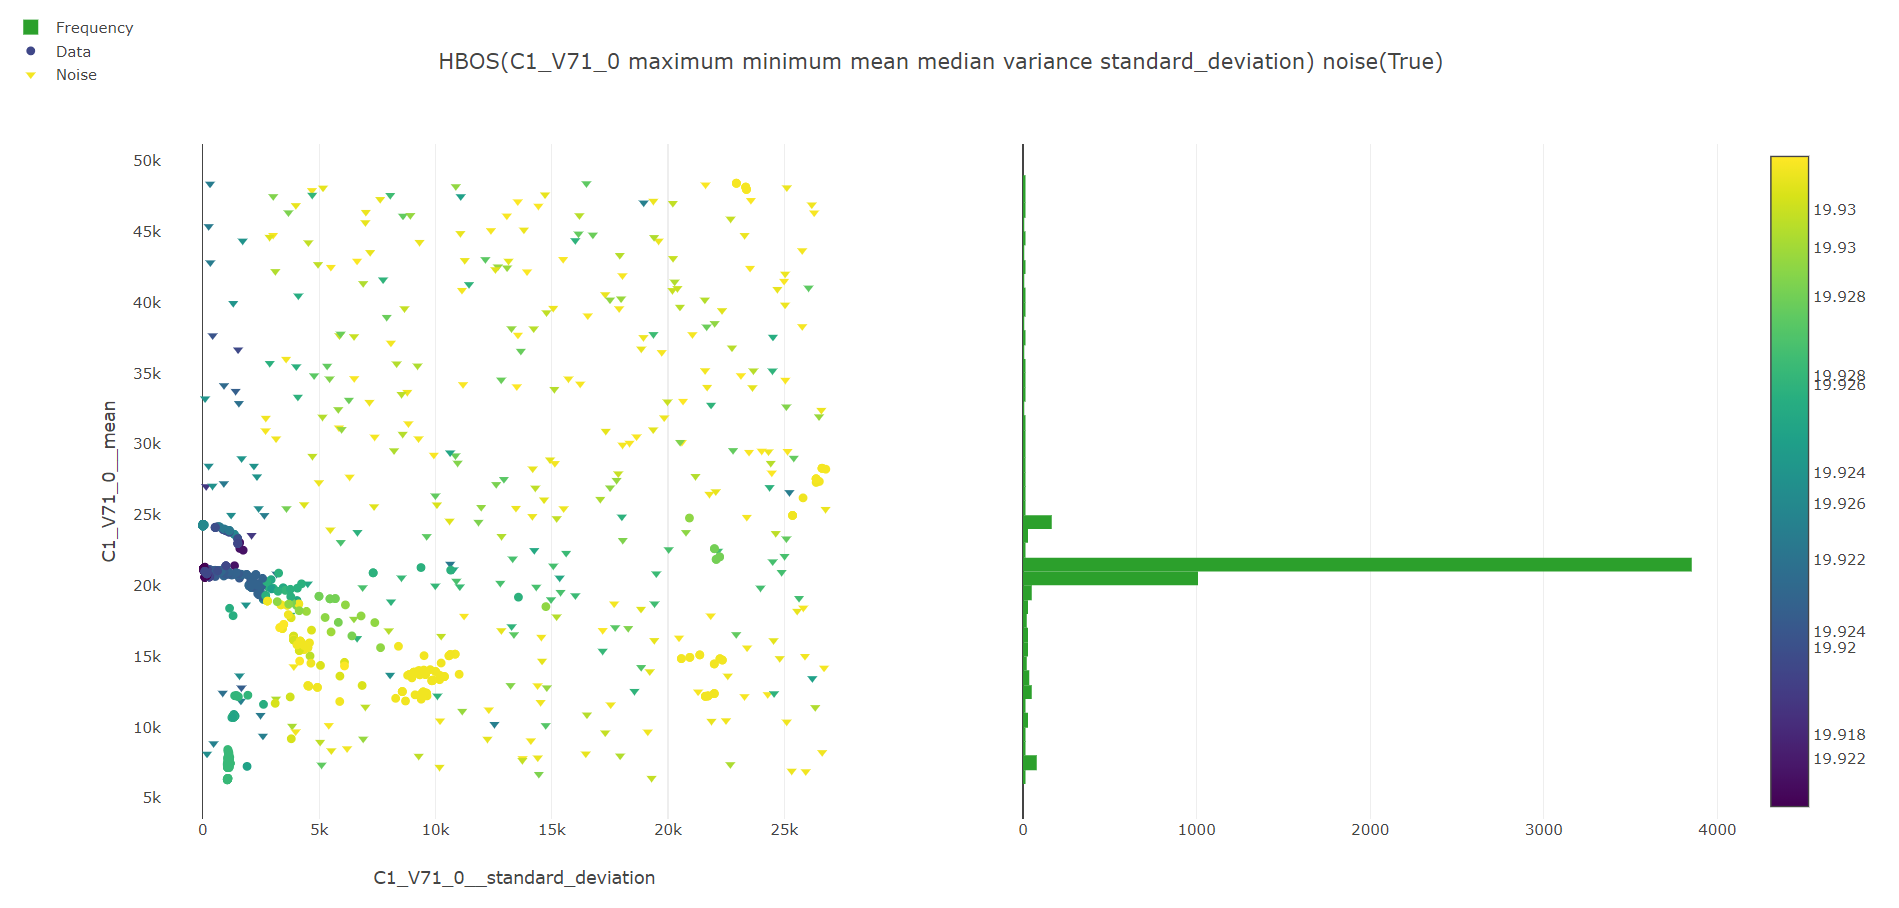
\includegraphics[width=\textwidth]{figures/vis3}
	\caption[Grafico dello score dei punti e del rumore usando HBOS e la variabile C1\_V71\_0]{Grafico dello score dei punti e del rumore usando HBOS e la variabile C1\_V71\_0. I punti verso il giallo sono più probabilmente outlier, mentre i punti verso il blu scuro sono più probabilmente inlier.
		
		\label{fig:vis3}}
\end{figure}


\subsection{Visualizzazione degli outlier con rumore a cluster}

Nella figura \ref{fig:vis4} il grafico mostra la classificazione degli outlier con l'aggiunta del rumore in 5 cluster casuali. Questa immagine conferma le conclusioni tratte alla fine della sezione \ref{AddestramentoEConfronto}, ovvero i cluster sono troppo distanti dai dati originali e troppo poco densi per poter confondere gli algoritmi di apprendimento. 

\begin{figure} [H]
	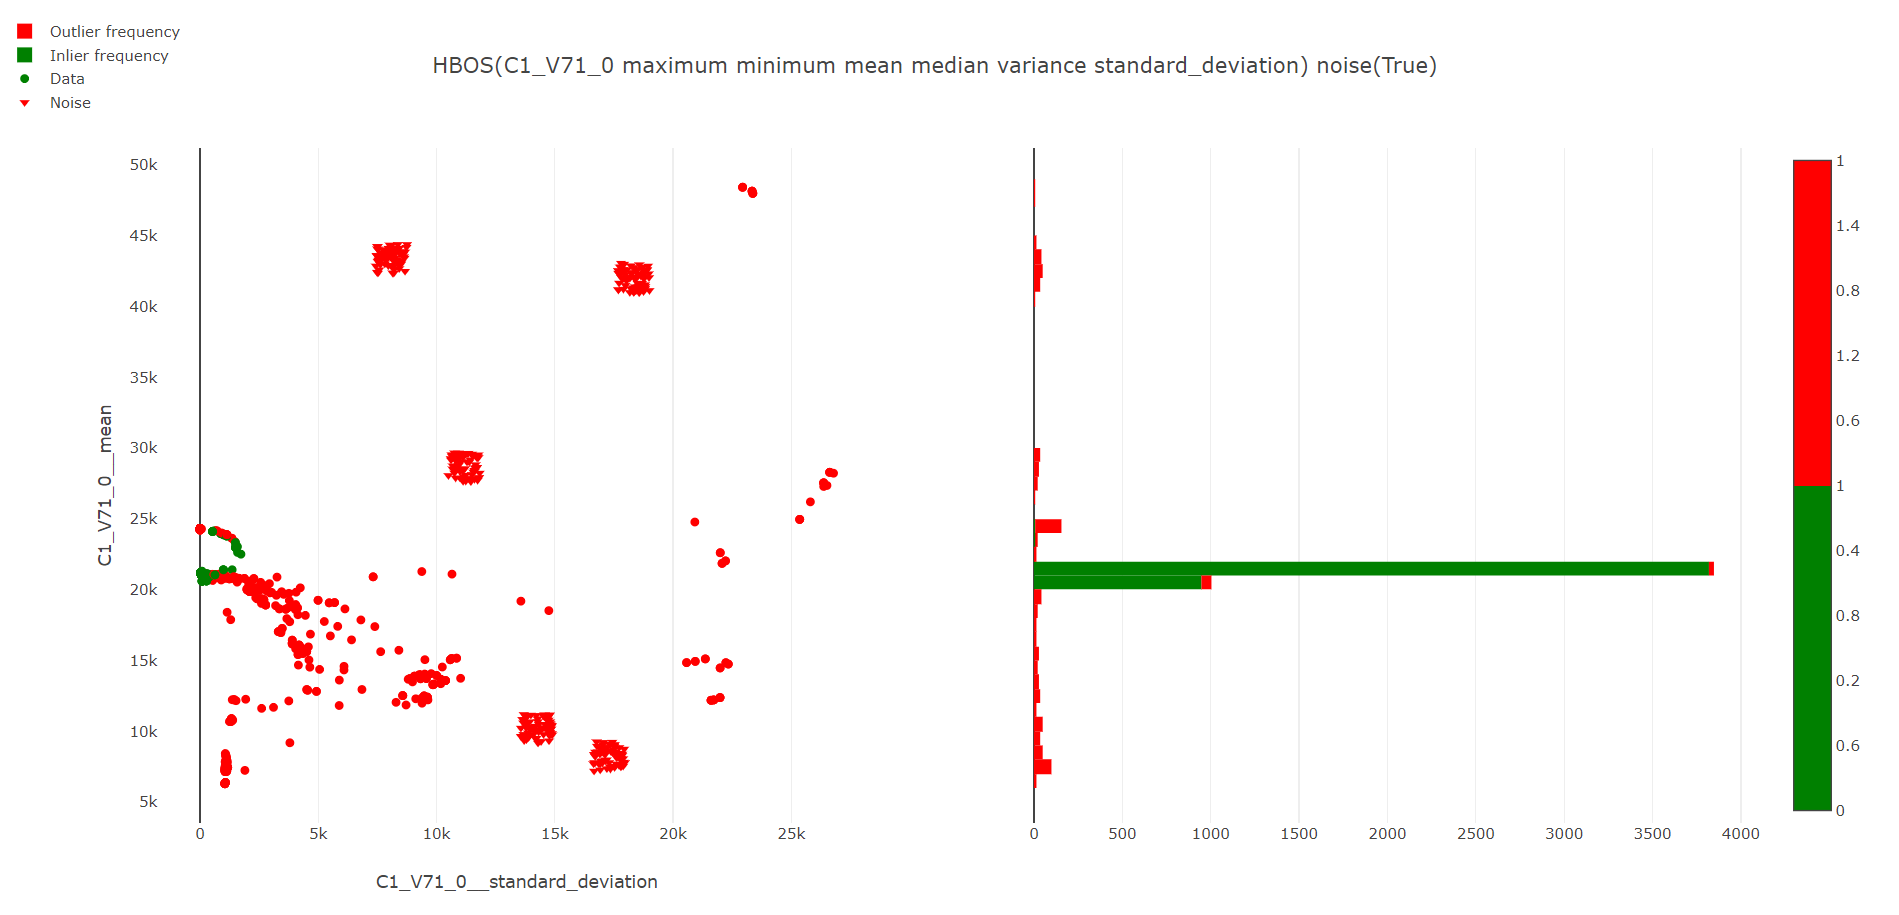
\includegraphics[width=\textwidth]{figures/vis4}
	\caption[Grafico degli outlier con aggiunta di rumore a cluster usando HBOS e la variabile C1\_V71\_0]{Grafico degli outlier con aggiunta di rumore in 5 cluster casuali usando HBOS e la variabile C1\_V71\_0. In rosso gli outlier, in verde gli inlier.
		
		\label{fig:vis4}}
\end{figure}


\subsection{Visualizzazione della decision surface}
La decision surface divide la superficie in più zone, ognuna delle quali rappresenta la probabilità che un punto in quella zona sia un'anomalia. Come si vede in figura \ref{fig:decision_surface} le zone rosse indicano che un punto in quelle zone è molto probabilmente un'anomalia, punti nelle zone blu sono comunque classificati come outlier ma è probabile che non lo siano. 

La linea tratteggiata rossa rappresenta la "decision boundary" ovvero il perimetro all'interno del quale i punti sono classificati come inlier. Per visualizzare meglio la decision surface, in figura \ref{fig:decision_surface} viene mostrata solo una parte del set di dati usato. 

Inoltre si possono notare le differenze tra i cinque algoritmi in base alle decision surface che generano, ad esempio PCA estrae le due componenti principali e forma quindi un ovale, oppure HBOS genera una superficie squadrata perché considera gli istogrammi di frequenza dei due assi.

\begin{figure} [H]
	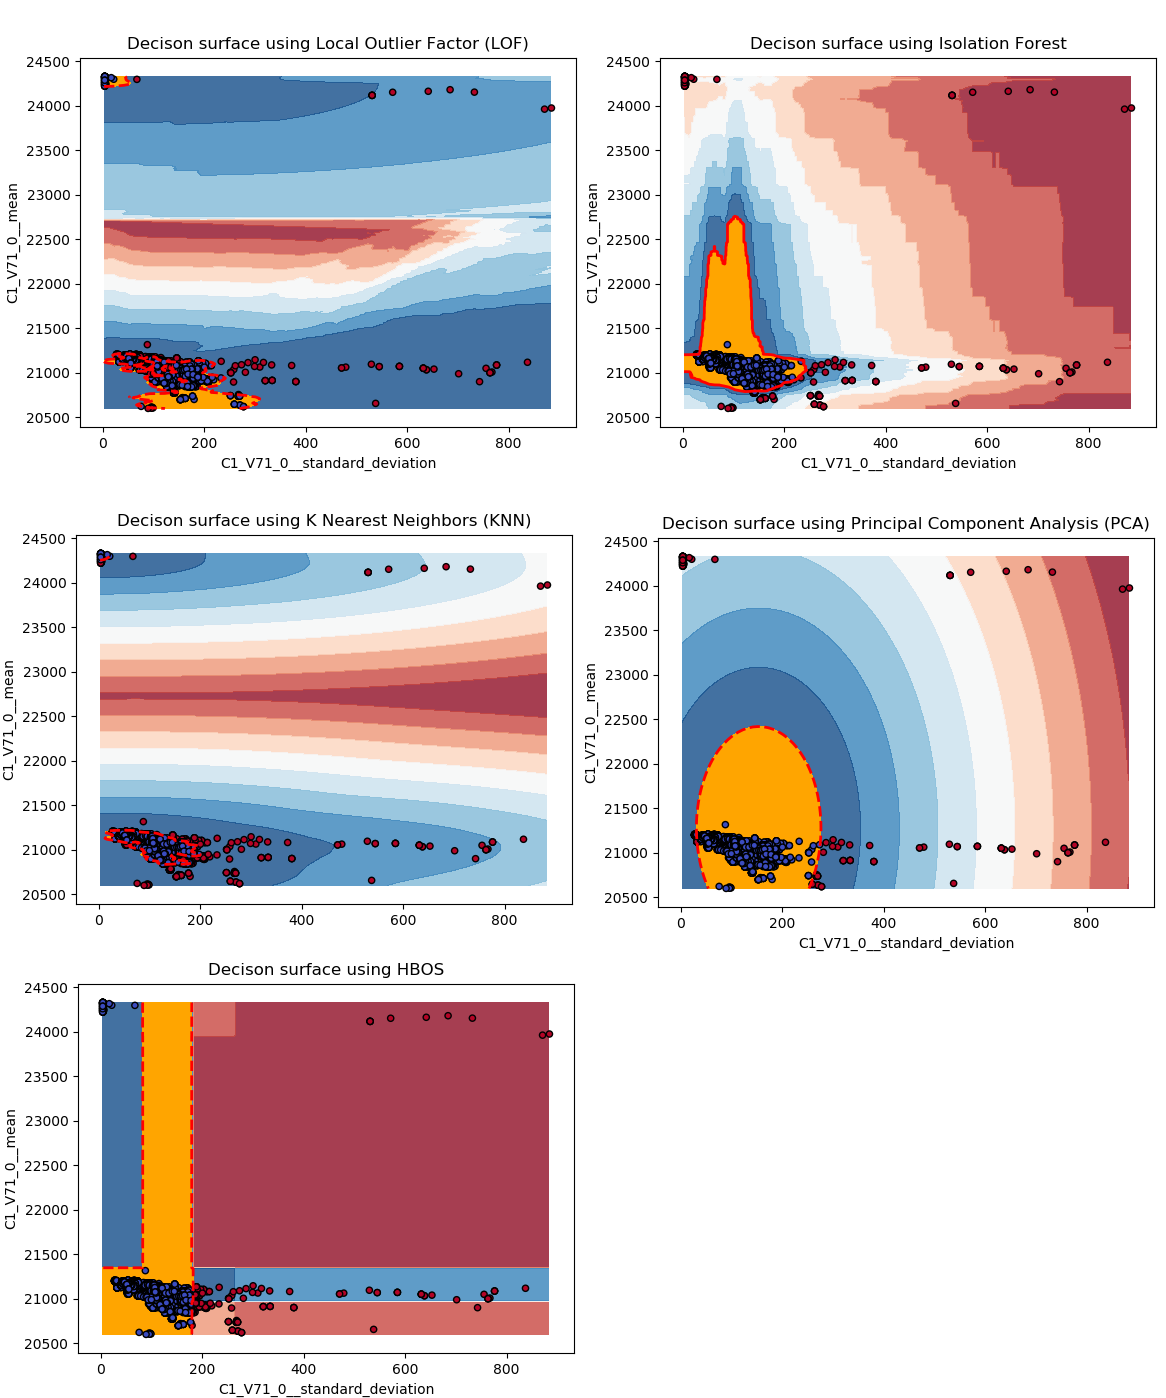
\includegraphics[width=\textwidth]{figures/decision_surface}
	\caption[Decision surface degli algoritmi]{Decision surface dei cinque algoritmi, le zone rosse indicano che un punto in quelle zone è molto probabilmente un'anomalia, punti nelle zone blu sono comunque classificati come outlier ma è meno probabile che lo siano. I punti all'interno della linea tratteggiata rossa sono inlier.
		
		\label{fig:decision_surface}}
\end{figure}

